%!TeX spellcheck = en-GB

%Basics
\documentclass[aps, prb, a4paper, english, 12pt, twocolumn, longbibliography, amsmath, amssymb]{revtex4-1}
\usepackage[utf8]{inputenc}
\usepackage{babel}

%Symbols and scientifics
\usepackage{amsmath, amsfonts, amssymb, bm}
\usepackage{physics}
\usepackage{mathtools}
\usepackage{siunitx}
\sisetup{
per-mode = fraction ,
round-mode = figures ,
round-precision = 3 ,
scientific-notation = engineering ,
output-decimal-marker = {.} ,
exponent-product = \times ,
separate-uncertainty = true ,
uncertainty-separator = \ ,
output-product = \cdot ,
quotient-mode = fraction ,
range-phrase = - ,
range-units =  single ,
inter-unit-product = \ensuremath{{\cdot{}}} ,
number-unit-product = \ ,
multi-part-units = single ,
}

%Appendix, TOC and Bibliography
\usepackage{appendix}
\renewcommand\appendixtocname{Appendices}
%\usepackage[nottoc]{tocbibind}
\usepackage[lastpage,user]{zref}

%Figures
\usepackage[svgnames]{xcolor} % Required to specify font color
\usepackage{float}
\usepackage{graphicx}
\usepackage{subcaption}
\usepackage{caption}
\usepackage{wrapfig}
\usepackage[a4paper, centering, rmargin=2.5cm, tmargin=2.5cm, lmargin=2.5cm, bmargin=2.5cm]{geometry}
\usepackage{etoolbox}
\usepackage{verbatim}
\usepackage[space]{grffile}
\usepackage[final]{pdfpages}
\usepackage{array}
\usepackage{multirow}
\usepackage{dcolumn}
%\usepackage{animate}
\usepackage{fontawesome}

%Header footer
\usepackage{fancyhdr}
\pagestyle{fancy}
\lhead{F. G. Kristensen,\\C. V. Sørensen og R. K. F. Wiuff}
\chead{Nanomechanics of graphene membranes\\}
\rhead{10/1-2018\\Course 34029: Physics Project}
\cfoot{Side \thepage\, af \zpageref{LastPage}}
\renewcommand{\headrulewidth}{0.4pt}
\renewcommand{\footrulewidth}{0.4pt}

%Text tools
\usepackage[super]{nth}
\usepackage[normalem]{ulem}
\usepackage{import}
\usepackage{url}
\usepackage{lipsum}
\usepackage{microtype}
\usepackage{hyperref}
\hypersetup{
  colorlinks   = true, %Colours links instead of ugly boxes
  urlcolor     = blue, %Colour for external hyperlinks
  linkcolor    = blue, %Colour of internal links
  citecolor   = red %Colour of citations
}
\usepackage[capitalise]{cleveref}
\usepackage{enumitem}
\usepackage{booktabs}
\usepackage{silence}
\WarningFilter{revtex4-1}{Repair the float}

%Python
\usepackage{minted}
\setminted{fontsize=\small}
\usemintedstyle{monokai}
\renewcommand{\listoflistingscaption}{Listings}

%Definitions and new commands
\newcommand{\logas}[1]{\log_{_{10}}{\left( #1 \right)}}
\newcommand{\sins}[1]{\sin{\left( #1 \right)}}
\newcommand{\tans}[1]{\tan{\left( #1 \right)}}
\newcommand{\coss}[1]{\cos{\left( #1 \right)}}
\newcommand{\sinas}[1]{\sin{\left( #1 \degr \right)}}
\newcommand{\tanas}[1]{\tan{\left( #1 \degr\right)}}
\newcommand{\cosas}[1]{\cos{\left( #1 \degr\right)}}
\newcommand{\lnas}[1]{\mathrm{ln}\left( #1 \right)}
\newcommand{\degr}{^{\circ}}
\newcommand{\me}{\mathrm{e}}
\newcommand{\eula}[1]{ \dpd{L }{#1} - \dod{}{t}\left(\dpd{L}{\dot{#1}}\right)}

%PDFPages and RevTeX incompatability fix
\makeatletter
\AtBeginDocument{\let\LS@rot\@undefined}
\makeatother

\begin{document}
%Titlepage herunder:
\begin{abstract}
 \begin{description}
  \item[Abstract] This paper analyses simulated vibrational modes in nanomembranes between 1 and 5 nm, using Atomistix Toolkit\cite{QuantumWise}, with the purpose of characterising the frequency response of the membrane, along with atomic behaviour of a few localised modes as to obtain a correlation with findings of similar computational simulations of microscale membranes.\cite{Davidovikj2016}. The nanomembranes in question is both a theoretical single layer idealised membrane and a more realistic double layered membrane, imitating a graphene layer upon a substrate. We hypothesised that the findings of such similar simulations will correlate in behaviour when moving to the nanoscale.
  As it turns out, the modes do scale, as the membrane sizes reduce to the nanoscale, and the frequencies and atomic movement are easily obtained using our developed analysistools. We discuss that our findings motivates to experimental tests on the nanoscale. Such membranes could be setup using nanomesh substrates with a graphene layer attached. These membranes could be produced using block copolymer lithography for the substrate and CVD for the graphene layer.
 \end{description}
\end{abstract}

\title{Nanomechanics of graphene membranes}
\date{10/1-2018}
\author{Frederik Grunnet Kristensen (s164003)}
\email[E-mail at ]{s164003@student.dtu.dk}
\author{Christoffer Vendelbo Sørensen (s163965)}
\email[E-mail at ]{s163965@student.dtu.dk}
\author{Rasmus Kronborg Finnemann Wiuff (s163977)}
\email[E-mail at ]{s163977@student.dtu.dk}
\affiliation{Technical University of Denmark}
\homepage[Homepage of the Technical University of Denmark ]{http://www.dtu.dk/english/}
\homepage[\\\faGithub \ Project Code Repository: ]{https://github.com/rwiuff/Nanomechanics-for-graphene-membranes}

\maketitle

\pagenumbering{arabic}

\tableofcontents

% ToC before List-ofs fix
\makeatletter
\let\toc@pre\relax
\let\toc@post\relax
\makeatother

\thispagestyle{empty}
\newpage
\setcounter{page}{1}

%Text
\section{Introducing the project}
% !TEX root = ../Main.tex

Since the isolation and characterisation of
Graphene in 2004 by Andre Geim and
Konstantin Novoselov, scientists have marvelled over the physical properties and potential
application of Graphene. Being a relatively new material, many aspects and ideas are being
investigated and researched at all times. Graphene yield extreme tensile strength as well as
extreme electric conductivity, yet its structure is fairly simple. Graphene consists solely of
carbon atoms thus making it easy to simulate using specialised software, since carbon atoms are greatly understood in terms of chemical
bonding.
As graphene is a very versatile material the possibilities for research in simulation enviroments are virtually limitless.
Therefore it is basically possible to make experiments limited only by imagination, in order
to discover new properties and possible applications of graphene. This saves resources
before entering the lab, where the simulated reality is tested.

In this rapport we will simulate and analyse the properties of nanomembranes as done in the papir "Visualizing the Motion of Graphene Nanodrums"\cite{Davidovikj2016}, which Figure \cref{Motivation} stems from. It shows how phonos travel through this membranes. However there this article,as many others, focuses on membranes in the micro-scale we will examine if this same phenomenons are found at the nano-scale. To do this we start by considering at ideal system of just one sheet of carbon atoms.
To make a more praticel membrane we will investigate if you can create the same membrane effects if you take a graphene layer and put it on top of a substrate with different sized and shaped holes, to form
form this nanomembrane and this is the that we will be looking at. It is expected possible to create such a nanomembrane at the
size of few tens of nanometers at Nanotech with Block-copolymer lithography or TEM
structuring of a substrate. In a virtual environment, it is possible to simulate phonons
in the graphene atop of these holes in the membrane. The purpose of this project is to
simulate phonons in the nanomembrane and find the optimal conditions for producing
phonons in the terahertz spectrum.
We will employ the software Atomistic ToolKit (ATK) to calculate phonon properties
of membranes as well as performing molecular dynamics of the excited membrane. The
software will enable prompt setup of relevant structures so that more time is free to analysis
and actual simulations.
\begin{figure}
    \centering
    \includegraphics[width=0.5\textwidth]{Figures/NanoDrums.png}
    \caption{Visualizing resonant motion. (a–h) Top, experimental data; bottom, finite-element calculation. The modes predicted by the calculation are indexed by (m,n). Panels b and c show that the nanodrum hosts a split degenerate (1,1) mode, while also the (2,1) mode is split, as is shown in panels d and e. The displacement profile measured in panel f resembles a (0,2) mode, which is distorted due to an imperfection as discussed in the main text. Panels g and h reveal a degenerate (1,2) mode. Scale bars: 1 $\mathrm{\mu m}$.\cite{Davidovikj2016}}
    \label{Motivation}
\end{figure}
\section{Introduction to Lattice Geometry, Nanomechanics and Atomistix ToolKit}
% !TEX root = ../Main.tex

\subsection{Lattice Geometry}
In order to set up the simulation environment the basic geometry of system must be defined. Using generating vectors as well as unitcells the structure and holes of the graphene sheet will be defined within this geometry.
\subsubsection{Bravais Lattice \& Generating Vectors}\label{BLGV}
At first we want to specify a Bravais lattice for the graphene-layer. The Bravais lattice is a lattice that is invariant under translation which means that the lattice does not change when you translate it with the vector
\begin{equation}
 \mathbf{T}=n\mathbf{a_{1}}+m\mathbf{a_{2}}\ \ \ \mathbf{a_{1}},\mathbf{a_{2}} \in \mathbb{R}^{2}
\end{equation}
Where $n,m \in \mathbb{Z}$ and $\mathbf{a_{1}}$, $\mathbf{a_{2}}$ are the generating vectors for the space lattice. Moreover, all the points in the lattice are given by
\begin{equation}
 \mathbf{R}=(nd,md)
\end{equation}
where $d$ is the spacing between the lattice points and $n,m$ can be both positive and negative integers. \\
As we are working with graphene which is carbon atoms arranged in a hexagonal structure, we want to choose a hexagonal Bravais lattice and define our generating vectors accordingly. Both generating vectors start at the center of a hexagon. This gives the generating vectors $\mathbf{a_{1}}=(d,0)$ \& $\mathbf{a_{2}}=\left(-\dfrac{d}{2},\dfrac{\sqrt{3}d}{2}\right)$. In \cref{hexagon} a drawing of the lattice with its generating vectors is shown.\\
As the carbon-carbon bondlength in graphene is \SI{1.42}{\angstrom}, the distance between the lattice points  in the Bravais lattice is $d=\SI{2.4612}{\angstrom}$. This gives the numerical form of the analytical derived expression for the generating vectors  $\mathbf{a_{1}}$ \& $\mathbf{a_{2}}$. \\
$\mathbf{a_{1}}=(\SI{2.4612}{\angstrom},0)$ \& $\mathbf{a_{2}}=\left(-\SI{1.2306}{\angstrom},\SI{2.1315}{\angstrom}\right)$. \\These are the vectors that will be employed during simulation.
\begin{figure}
 \centering
 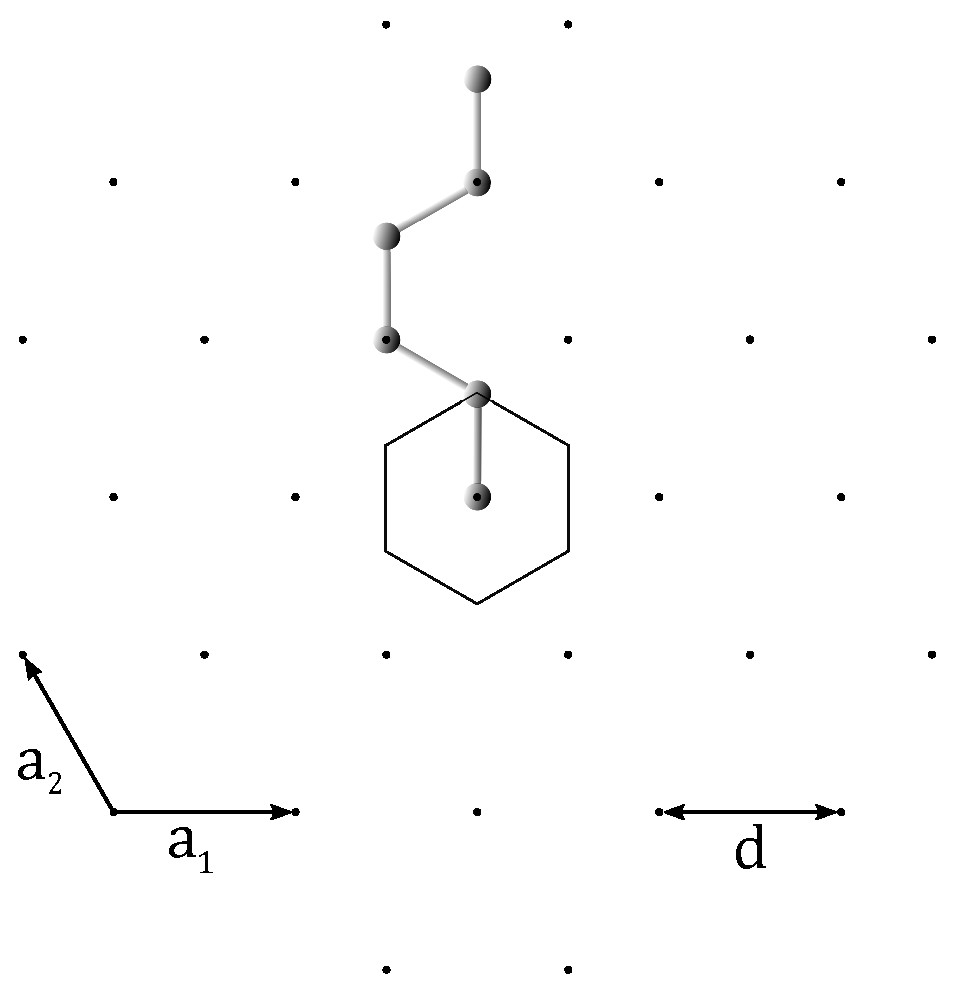
\includegraphics[width=0.5\textwidth]{Figures/hexagon2.eps}
 \caption{Hexagonal Bravais lattice structure with generating vectors $\mathbf{a_{1}}$ \& $\mathbf{a_{2}}$. The Hexagon in the middle with the solid lines is unit cell and the shaded elements are the carbon atoms placed in the lattice.}
 \label{hexagon}
\end{figure}

% !TEX root = ../Main.tex

\subsection{Nanomechanics}
This following section will focus on the mechanics of the know defined geometry of the Graphene sheet. It will incorporate boundary conditions in two dimensions, Hooke's law, the normal modes of the lattice as well as phonons. (relaxation energy)

\subsubsection{Boundary Conditions in Two Dimensions}
\todo[inline]{Write section}
 
\input{sections/MD.tex}
\subsection{Atomistix ToolKit: ATKPython and Nanolanguage}
The Python script creating the lattice and tags are printed and commented in the Appendix on \cpagerefrange{NSCstart}{NSCend}

\section{Simulating vibrating membranes}
% !TEX root = ../Main.tex

\subsection{Our Workflow}
In order to simulate the vibrational modes in a graphene lattice, the dynamical matrix needs to be, both calculated and postprocessed. Both of which needs substantial amounts of computational power and time. The workflow is therefore created with steps of scripts which can be sent to a hpc cluster for computation.
The workflow for simulating a graphene sheet is described as such:
\begin{enumerate}
  \item Create the sheet in question with \textbf{NanoSheetCreator.py} (\labelcref{NSCS}).
  \item Use VNL Builder GUI to ensure correctly tagged holes.
  \item Use \textbf{00\_FixConstraints.py} (\labelcref{00}) to fix the tagged atom indices\footnote{Due to a bug in ATKPython some numpy manipulation of the atomic bulk configuration was needed. See \cref{00}}.
  \item Use \textbf{01\_RelaxSheet.py} (\labelcref{01}) to optimise the bond length and geometry of the graphene sheet.
  \item Use \textbf{02\_DynamicalMatrix.py} (\labelcref{02}) to compute the Dynamical Matrix for the sheet.
  \item Use \textbf{03\_SheetVibrations.py} (\labelcref{03}) to find calculate the vibrational modes of the sheet.
  \item \todo{Insert Analysis tools}
\end{enumerate}
Flowchart is shown on \cref{fc}.
\todo[inline]{Insert flowchart here}

% !TEX root = ../Main.tex
\subsection{\faGithub \ Code Repository and code compendium}
All of the mentioned code and scripts exists as a repository available online:\newline
\url{https://github.com/rwiuff/Nanomechanics-for-graphene-membranes}
Beware that ATKPython is required to run the scripts.
The code can also be found in the Code Compendium in \cref{CoCo}.

\subsection{NanoSheetCreator.py and NanoMembraneCreator.py}\label{NSCS}
The first script generates the graphene membrane with atoms tagged in a hexagonally shaped path. The output is the sheet in the \textit{.hdf5} format.

The workings of the script is briefly described as such:
First the script creates a bravais-lattice consisting of a hexagonal unit cell. Then two carbon atoms are placed in the unitcell and the unit cell is repeated to the users specifications. \cref{2435} demonstrates, by example from NanoSheetCreator.py, how such lattice is created with Nanolanguage.
\onecolumngrid

\begin{listing}[H]
 \inputminted[python3=true,bgcolor=Black,linenos=true,firstline=24,lastline=35]{python}{Listings/NanoSheetCreator.py}
 \caption{Lines 24-35 from the NanoSheetCreator.py shows how Nanolanguage can be used to create a hexagonal bravais lattice}
 \label{2435}
\end{listing}
\twocolumngrid
The user is then asked to input position and size of the hexagonal tag wanted for placement of the hole. Lastly the sheet can be repeated and information about the position and sizes of the tags are printed to a \textit{.txt} file.

\subsection{00\_FixConstraints.py}\label{00}
A historical bug in ATKPython demands consecutive indices for constrained atoms when using the function \textit{phononEigensystem}. Thus a script was written to ensure that tag with these indices were consecutive. Furthermore, when working with two layer membranes, the script tags the individual layers as "Layer1" and "Layer2".

\subsection{01\_RelaxSheet.py and 01\_LennardJonesRelax.py}\label{01}


\subsection{02\_DynamicalMatrix.py}\label{02}
\subsection{03\_SheetVibrations.py}\label{03}

\onecolumngrid

\begin{figure}[H]
    \centering
    \includegraphics[width=\columnwidth]{Figures/NanoLayer5nm.png}
    \caption{A snapshot from ATK\cite{QuantumWise} showing how the clamped system looks like when at rest. The hexagon in the middle is marked with tags and is the only part of the sheet that is not constrained i.e. the free standing membrane.}
    \label{fig:clamped}
\vspace{12em}
    \centering
    \includegraphics[width=\columnwidth]{Figures/DoubleMembrane.png}
\caption{The picture on top shows the two layer system from above. The one on bottom shows the system from the side. Both snapshots have been taken in ATK\cite{QuantumWise}.}
\label{interlayersys}
\end{figure}
\twocolumngrid

\section{Data extraction and analysis}\label{DEA}
\subsection{Clamped System}
This following section focuses on data extraction and analysis for a system of graphene with a free standing hexagon in the middle of a clamped graphene sheet. The free standing hexagon will therefore be equivalent to a hole in the graphene sheet.  
\subsubsection{Frequency vs. hole size}
In order to find the correlation between frequency of the modes in the hole and the hole size, the frequency over each free standing hexagon, which varies in size, is extracted and plotted as a function of the size of the given hole. \\
This is done by defining a sheet of a definite size in VNL and thereafter check the frequencies for the different holes by inserting the different size holes, one after the other. The distance from the edge of the hole, to the edge of the sheet (or the next hole) is called "neck" and has been chosen to be 5 nm for the biggest hole which has a 10 nm diameter. \\
Furthermore, only the frequencies for the first 10 modes will be checked. 
\section{Discussion}
% !TEX root = ../Main.tex
\subsection{Size vs Frequency}
The 
\subsection{Interlayer interaction}

\subsection{Compare and discuss results from other journals}

\subsection{Whats next?}

\subsection{Perspective: Going from theory to the lab}

\begin{figure}
  \centering
  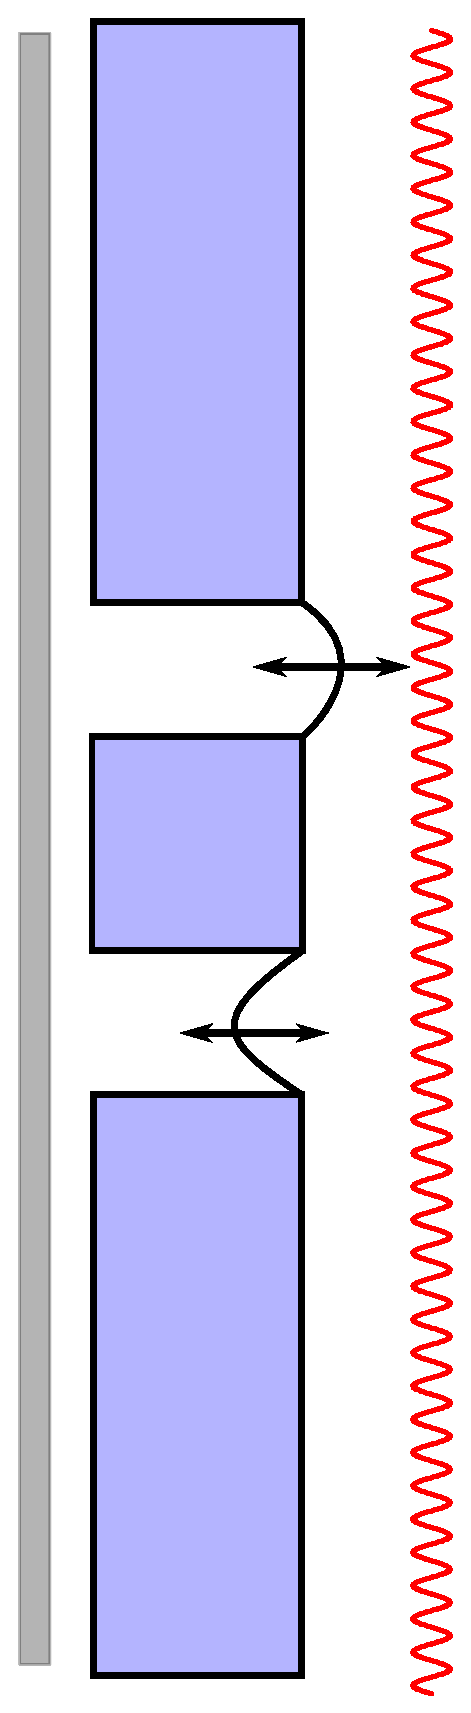
\includegraphics[width=0.3\columnwidth]{Figures/Fuck_dig_christoffer.eps}
  \caption{The setup of our proposed experiment, with the supstrakt (blue), the laser (red), the conductor (gray) and the membrane(black)}
  \label{FDC}
\end{figure}
\section{Conclusion}
% !TEX root = ../Main.tex
Through our analysis of the both the clamped system and the two layer system we conclude that the membranes respond well to the frequencies at nano scale and that the atomic behaviour of the modes correlated with the findings of similar simulations on micro scale membranes. The response frequencies for modes at nano scale were found to be in the Terahertz spectrum, which further motivates experimental tests. Because of these findings it reasonable to believe that a nano device which uses the membranes as gates, can be created. 
\begin{acknowledgments}
We would like to thank Tue Gunst and Mads Brandbyge at DTU Nanotech for their guidance and help.
\end{acknowledgments}
%End of text

%Bibliography herunder:
\newpage
\onecolumngrid
\bibliography{Physics-Project-Nanomechanics-of-Graphene-Membranes}

\newpage
\listoffigures
\listoftables
\listoflistings
\newpage
%Appendicer herunder:
% !TEX root = Main.tex

\appendix
\appendixpage
\addappheadtotoc
%\section{Animation of \nth{9} mode}
%\begin{center}
%  \animategraphics[autoplay,loop,width=\textwidth]{60}{VNL/Frames/frame}{1}{60}
%\end{center}
%Section 1 herunder:

%Section 2 herunder:

\end{document}
